\section{BranchConnect: The Game}
\label{sec:game}
The online game is accessible by laptops and mobile touch devices, and many users can play at the same time.
The objective of the game is to collect valid layouts of branches which are fabricatable with 3 axis CNC milling machines.
By analyzing the connectivity of branches and target points, the game checks feasibility of a given layout.
Similar to our game, the work \textit{guidance system during furniture design} inspected connectivity, durability, and stability \cite{umetani2012guided}.
Unlike their work, our game puts emphasis on \textit{fabricatability}, as well as \textit{geometric connectivity}, and does not calculate structural performance of each joint.
%Instead, we limit valid layout space by selected joint conditions, and group conditions.
Instead we use simple geometric analysis to compute validity.
We also assume that every fabricated joint works as a rigid joint, thus single connection is counted as stable to hold a pair of branches.


%The workflow of the game is illustrated in Figure~\ref{fig:game_flowchart}.
%\begin{figure}[ht]
%  \begin{center}
%    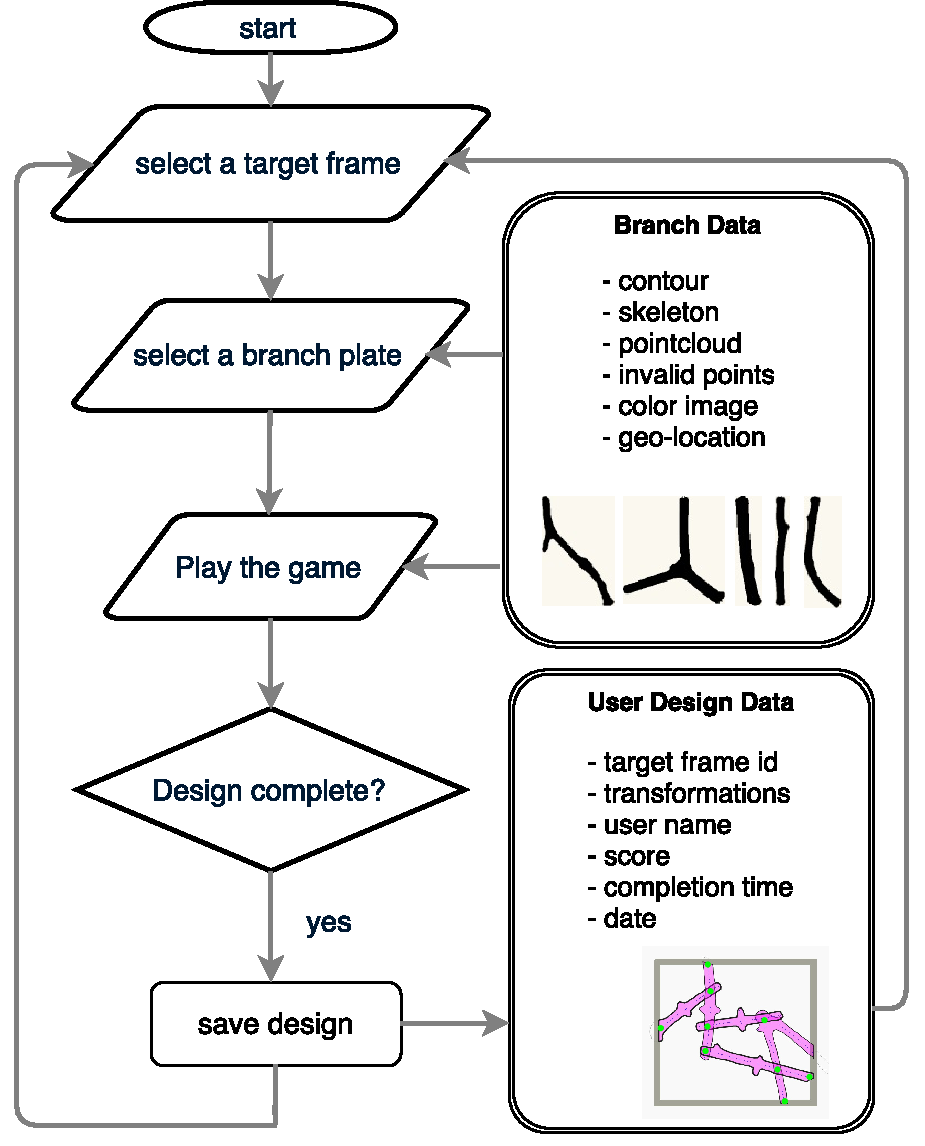
\includegraphics[width = 0.25\paperwidth]{images/system/systemFlowChart.pdf}
%    \caption{The workflow of \textit{BranchConnect}. Branch data and user design data are stored on cloud database.}
%    \label{fig:game_flowchart}
%  \end{center}
%\end{figure}

%Describing user experience, firstly a user selects a target frame indicating multiple target points to be connected, and then selects a set of branches fixed on a plate (the left in Figure \ref{fig:game_interface}).
Each frame comes with a set of predefined target points on it to be connected.
%A user selects a target frame and connect the assigned target points
The distribution of these target points is predefined by the system, and end users can not modify them.
After a user selects a target frame and a set of branches on a plate (Figure \ref{fig:game_interface} left), the user is guided to the game interface, consisting of the frame with the target points, and the set of available branches at the bottom (Figure \ref{fig:game_interface} right).
The user picks a branch from the available set on the bottom, and drag\&drop it to the inside of the target frame.
By selecting and dragging a branch, the user searches a good 2D pose through geometric manipulations such as move, rotate, and horizontal flip (or mirror).
A joint is created when an intersecting pair is detected, and the pair forms a group.
The group is used for evaluating connections between target points (\textit{Bridged}).
The conditions of joint and group are indicated with simple color-code.
%Once the user finishes positioning, score is updated with weighted sum of parameters.
Together with the color-code, the score update guides the user to form a valid design.
Within the limited number of branches, the goal is to bridge all the target points by connecting all the used branches in one group.
For higher scores, the user can keep modifying the design, and save it to the database.

\begin{figure}[ht]
  \begin{center}
    
\includegraphics[width = 0.4\paperwidth]{images/interface/game_interface.png}
    \caption{Left: the selection interface for target frames (top) and branch panels (bottom). Right: the start interface of the game.}
    \label{fig:game_interface}
  \end{center}
\end{figure}
%
\subsection{The Game System}
There are many physics simulation libraries for game, however, our game needs to detect intersected branch pairs, thus collision detection with physics engines is overkill for our browser game.
%Our game is running on browsers with rich 
Also, branches have free-form concave shapes, thus further geometric preparation such as convex decomposition is necessary for using these libraries.
For fast and robust intersection detection, our game extensively uses down-sampled skeletons of branches.

Hubbard and Philip developed collision detection by representing an object with hierarchical 3D spheres aligned on a skeleton \cite{Hubbard:1996:APS:231731.231732}.
Our game takes similar approach but limited in 2D, but more focused on searching fabricatable joints.
In the game, down-sampled skeletons are used to find the pair of closest skeleton points between two branches.
When a branch is selected, the system searches the closest skeleton point of the selected branch with other skeletons of available branches.
More precise joint calculation with high-resolution contours is further described in Section \ref{sec:fabrication}.




\subsubsection{Joint Condition}
\label{sec:joint}
Joint is the essential entity not only in the game but also in the fabrication process of customized lapped joineries.
Importantly, each pair of branches must have one flipped branch for fabrication constraint (Section \ref{sec:fabrication}).
Figure~\ref{fig:joint_condition} illustrates valid and invalid joint conditions.
Our joint only takes crossed pair (Figure~\ref{fig:joint_condition}.1) because they are structurally stable, relatively simple to fabricate, and creates diverse designs.
Tangential connections are counted as invalid as fabrication of tangential joinery is challenging with small branches (Figure~\ref{fig:joint_condition}.3).
A valid joint's angle stays within a fixed range (Figure~\ref{fig:joint_condition}.1 and 2).
Joints close to metal fixtures are also counted as invalid (Figure~\ref{fig:joint_condition}.4).
Valid and invalid joints are displayed with green and red respectively.

\begin{figure}[ht]
	\begin{center}
		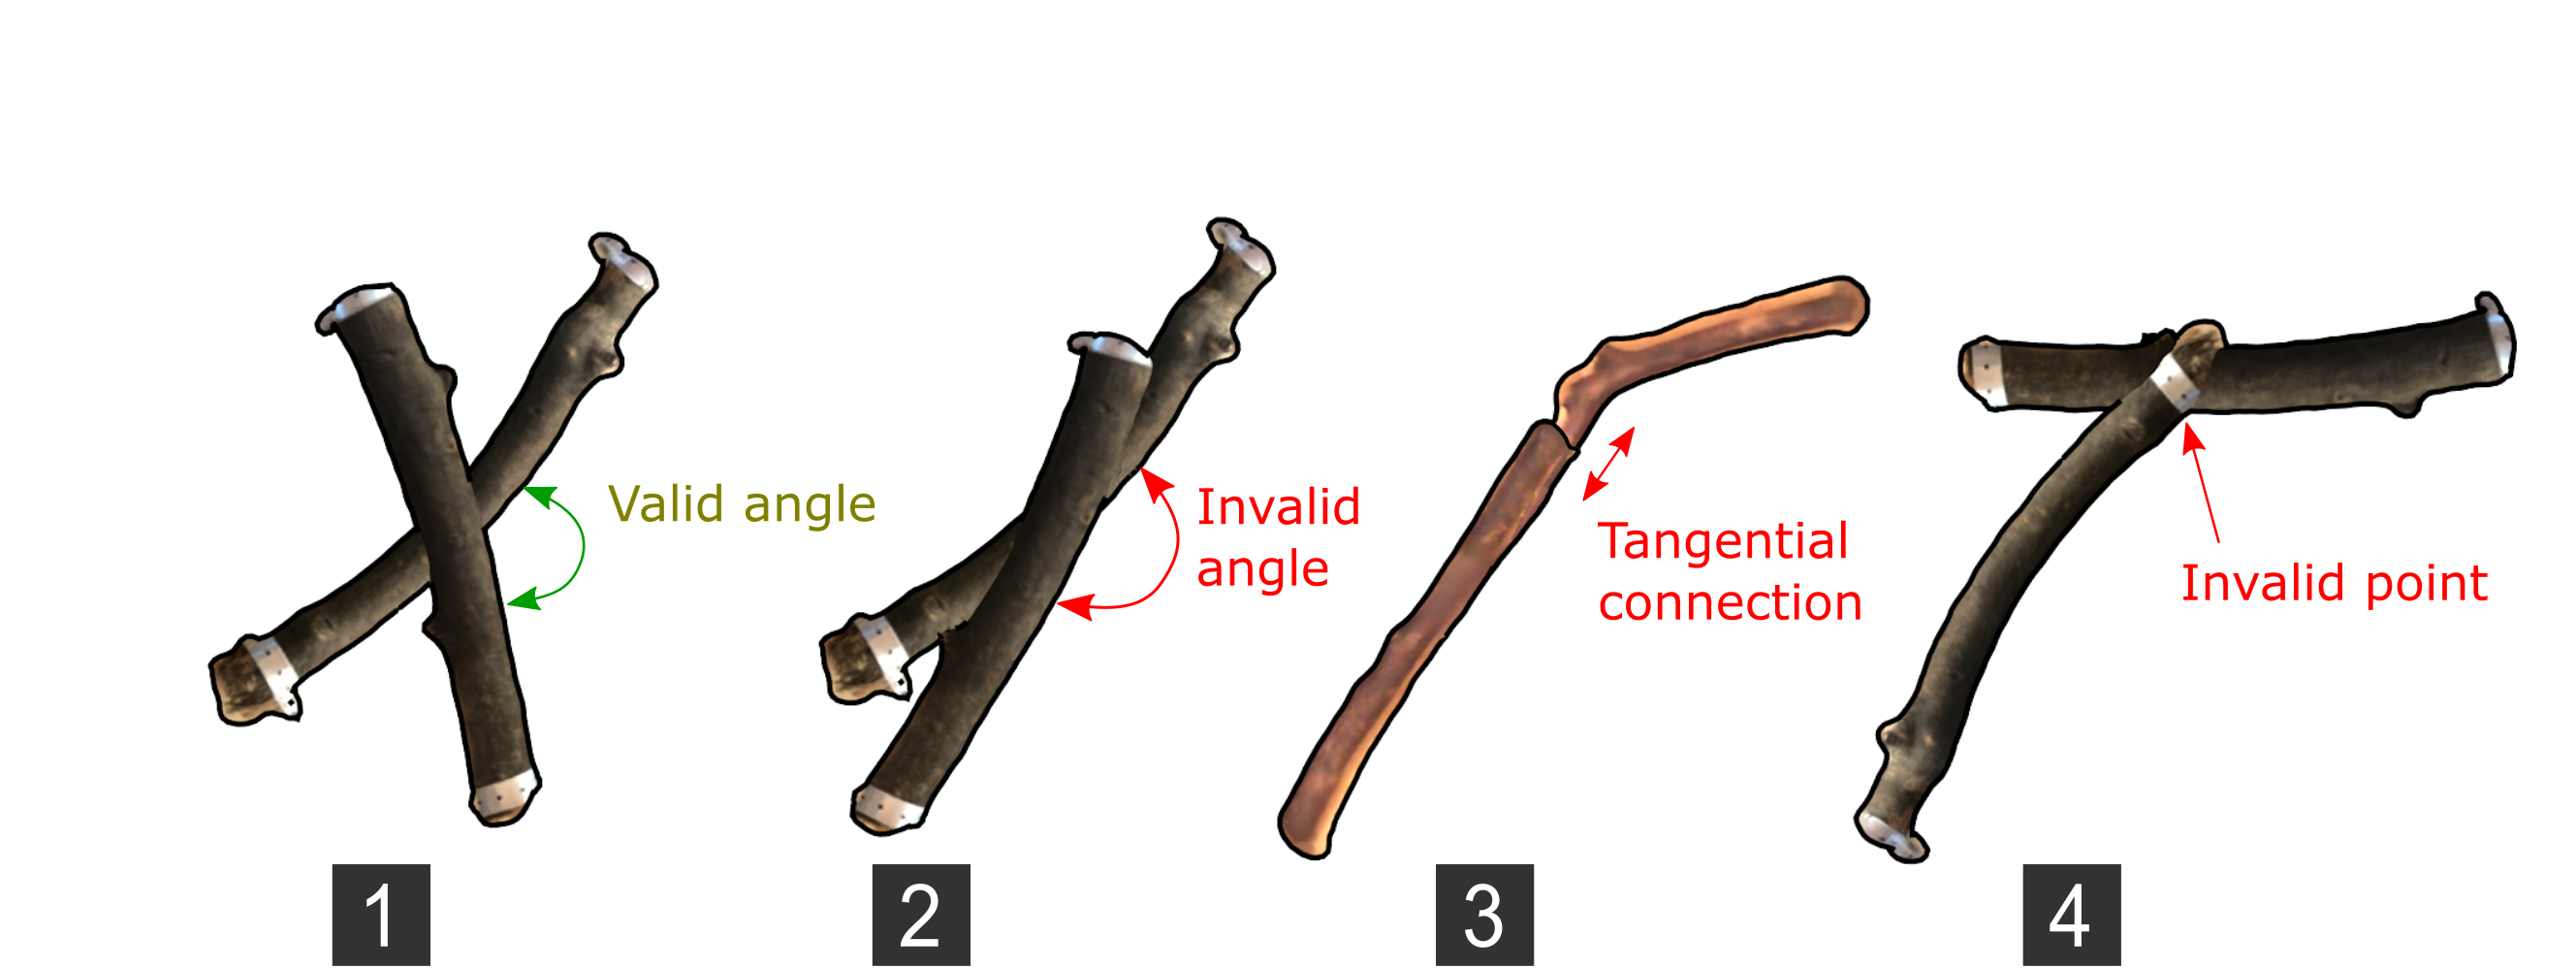
\includegraphics[width = 0.4\paperwidth]{images/system/joint_conditions_2.png}
		\caption{Joint conditions. 1. valid joint. 2. invalid for violating the angle. 3. invalid tangential connection. 4. invalid for connecting on a fixture point. }
		\label{fig:joint_condition}
	\end{center}
\end{figure}




To describe the joint update process, let each branch $b_i$ be a member of a set of the branches $\mathcal{B}$ dropped inside of the target frame by a user.
The user freely choose $\mathcal{B} \in \mathcal{B_{plate}}$, where $\mathcal{B_{plate}}$ is the branches fixed on a selected plate, denoted as $\mathcal{B_{plate}}$.
We accept one joint with a pair of branches, but a branch can have multiple joints with other branches. 
The process starts from the selected branch $b_i$ and updates joint conditions of the selected branch with paired branches.
When an intersected pair is detected, it stores $j$-th joint $j_{i, j}$ in $b_i$ with joint conditions (Figure~\ref{fig:joint_condition}).
After evaluation, as in Figure \ref{fig:joint_condition},  we have joint labeled as valid or invalid.
When a branch $b_i$ is connected to one of target points $t_j \in \mathcal{T}$, the target point $t_j$ is stored in $b_i$.
Note that we also take one target point for each branch.
This process as well as group condition update process are illustrated in Figure \ref{fig:system_flowchart}.

\begin{figure}[ht]
	\begin{center}
		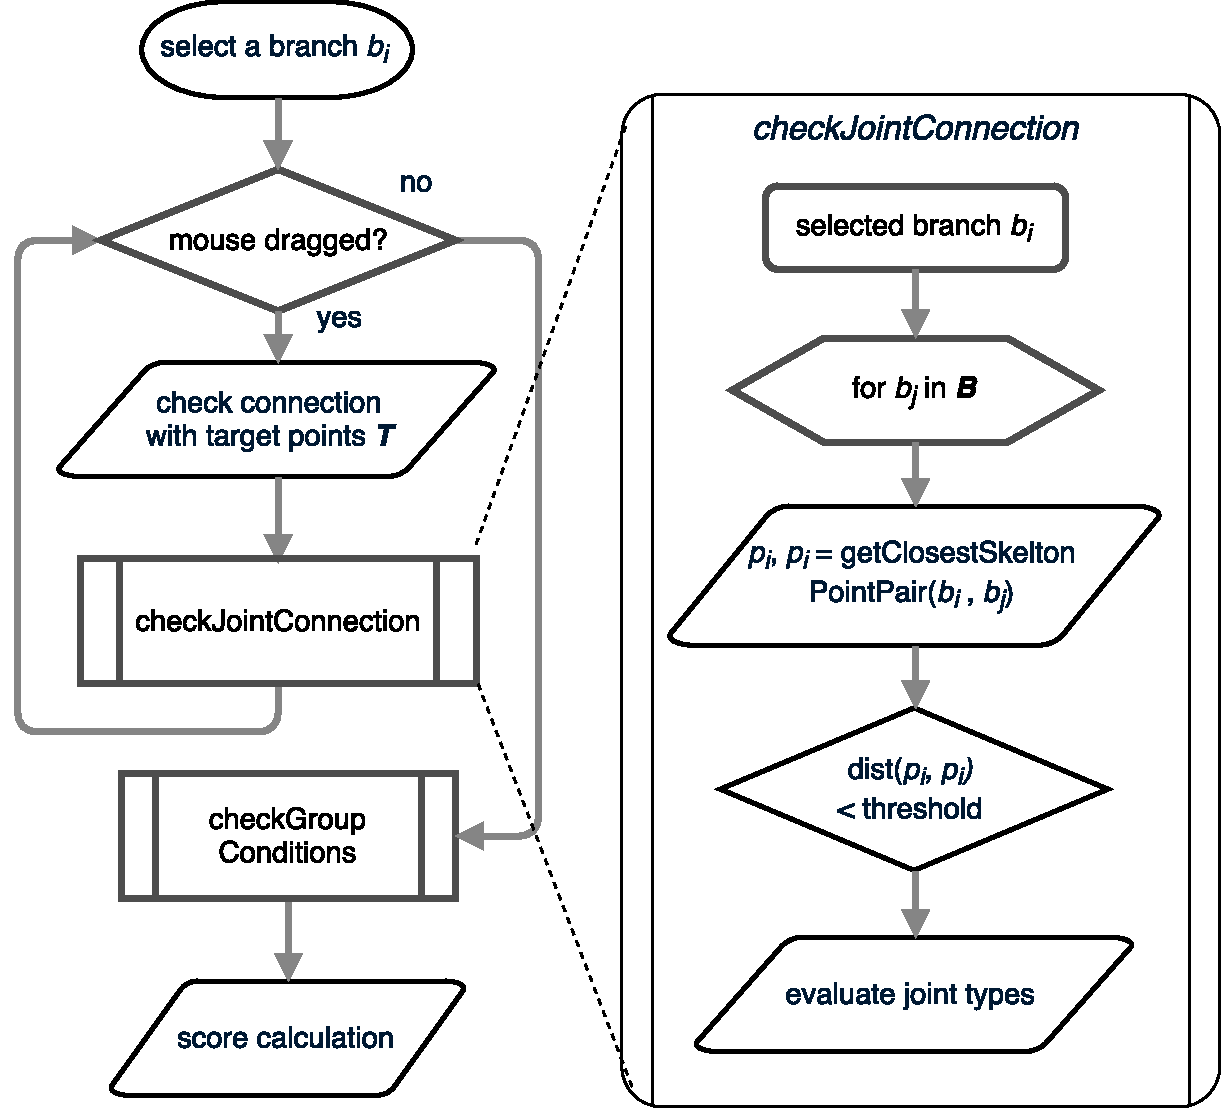
\includegraphics[width = 0.35\paperwidth]{images/system/closestPointAlgorithm.pdf}
		\caption{Left: an overview of the game system with 1.joint update 2.group update and 3. score calculation. This process is iteratively executed while a user is exploring layout by dragging a branch. The joint update process is further illustrated in the right, and group condition update is described in Algorithm \ref{al:connection}. }
		\label{fig:system_flowchart}
	\end{center}
\end{figure}

% well as the paired branch $b_{\text{paired},j} \in \mathcal{P}_{\text{paired},i}}$.



\subsubsection{Group Condition}

After updating joint conditions of all the paired of branches, the system updates the number of groups as well as its connection with the target points on a frame.
If a group is not connected to any target point nor other groups, the group is \textit{Islanded} and structurally invalid.
While a user is positioning a branch by dragging or rotating, groups are continuously calculated and indicated by simple color (Figure \ref{fig:group}).

\begin{figure}[ht]
  \begin{center}
    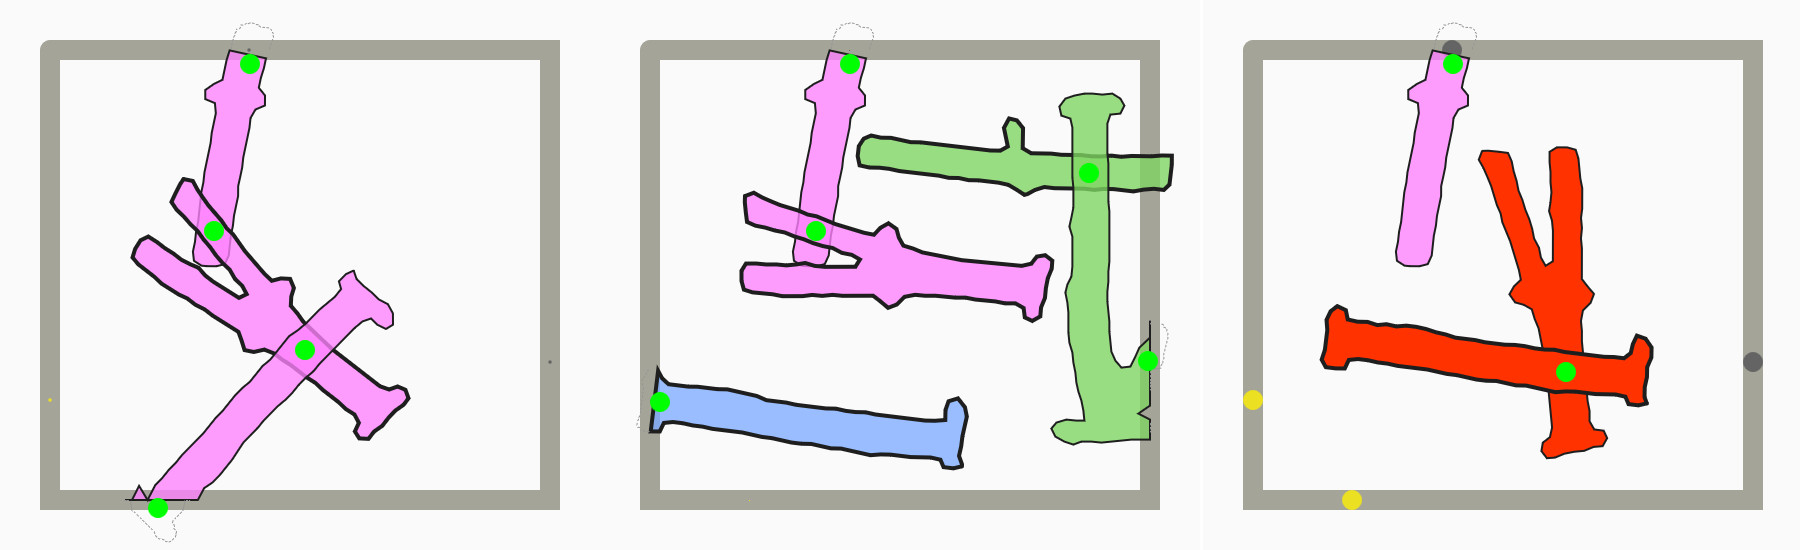
\includegraphics[width = 0.4\paperwidth]{images/interface/groups.jpg}
    \caption{Left: valid group with two target points connected. Middle: valid but three groups. Right: invalid due to the \textit{Islanded} situation. }
    \label{fig:group}
  \end{center}
\end{figure}


After all the joint conditions are updated, we evaluate group conditions.
Iterating $b_i \in \mathcal{B}$, the first group $g_0$ is created and stored as $b_0$.
When a branch is connected to a target point, the graphics of the point changes, and the branch and its belonging group's color also changes.
When a group bridges a pair of target points, a special score is added and displayed in a pop-up square, also the graphics of target point's changes.
The branch connected to the target point is trimmed at the target point, and the trimmed length is subtracted from the score.
%The other paired branch $b_{\text{paired},i}$ stored in $j_{\text{valid}, j}$ is used for tracing the connection with other paired branch in each valid joint $j_i$. \todo{incomplete sentence!}
The game is completed when the number of $\mathcal{G}$ is one, and all the target points are connected with the group.
The algorithm which checks group conditions is described in Algorithm \ref{al:connection}.

\begin{algorithm}
  \caption{Group Condition Update Algorithm}
  \begin{algorithmic}[1]
    \Function{UpdateGroups}{$\mathcal{B}$}
    \State{Reset all the groups $\mathcal{G}$ }
    \State{Create new group $g_0$}
    \State{$b_0 \text{ is added to } g_0$}
    \If{$b_0$ has connected target point $t_i \in \mathcal{T}$}
      \State{$g_0 \text{ sets } t_i$}
    \EndIf
    \State{$g_0 \text{ is added to }  \mathcal{G} $}

    \For{each branch $b_i$ in $\mathcal{B}$}
    \State{\textit{GroupConnection} $\gets false$}
      \For{each group $g_j$ in $\mathcal{G}$}
        \For{each branch $b_j$ in $g_j$}
          \If{ $b_{\text{paired},i} \in \mathcal{P_i}$ has $b_j$}
            \State{ $b_i  \text{ is added to } g_j $}
            \State{ \textit{GroupConnection}  $\gets true$}
            \If{($b_i$ has $t_i$) and ($g_j$ has $t_j$) }
              \State{ Set $g_j$ as \textit{Bridged}}
            \EndIf
            \If{$g_j$ has no $t_j$}
              \State{ Set $g_j$ as \textit{Islanded}}
            \EndIf
            \State {\textit{break}}
          \EndIf
        \EndFor
      \EndFor

      \If{ \textit{GroupConnection} is \textit{false} }
        \State{create new group $g_{new}$}
        \State{ $b_i  \text{ is added to } g_{new}$}
        \State{$g_{new} \text{ is added to }  \mathcal{G}$}
      \EndIf
    \EndFor

  \EndFunction
  \end{algorithmic}
  \label{al:connection}
\end{algorithm}

\subsubsection{Score Calculation}
We calculate the score with weighted sum of following entities: the numbers of valid and invalid joints on each branch, the number of groups as $N(\mathcal{G} )$, the number of islanded groups as $N(g_{\text{islanded}} \in \mathcal{G} )$, the number of bridged target points as $N(t_{\text{bridged}, i}) \in \mathcal{T} )$.
The trimmed lengths of branches which are connected with target points are denoted as $trimmed(t_j, b_i)$
The score is weighted sum of these joint and group conditions, denoted in Equation (\ref{eq:score}).
The weights $w_1 \dotso  w_5$ are non-negative weight coefficients pre-adjusted in advance by authors.


\begin{equation} 
 \begin{aligned}
 Score =  &\; w_1  \sum_{1}^{N(\mathcal{B})} \sum_{1}^{N(\mathcal{J}_{\text{valid},i})} j_{\text{valid}, j, i}
 + w_2  \sum_{1}^{N(\mathcal{B})} \sum_{1}^{N(\mathcal{J}_{\text{invalid},i})} j_{\text{invalid}, j, i}\\
+ &\; w_3  \sum_{1}^{N(\mathcal{G})} g_{\text{islanded}}
	 + w_4  \sum_{1}^{N(\mathcal{T})} t_{\text{bridged}}
+  w_5 \sum_{1}^{N(\mathcal{T})} trimmed(t_j, b_i)
 \\
   \textrm{s.t.} \; w_j  \geq  &\;0 \; \forall j \in 1, \dotsc , 5
 \end{aligned}
 \label{eq:score}
\end{equation}
